% Autor: Adina Wagner, 215486

%---------- Pakete und Dokumenteinstellungen -------------------------------------

\documentclass[a4paper, 12pt]{scrreprt}

\usepackage[ngerman, american]{babel}   %andersherum, also "ngerman, american" sind die Ueberschriften in Englisch
\usepackage[T1]{fontenc}			%Kodierung des Zeichensatzes
\usepackage[utf8]{inputenc}		%Dt. Umlaute mit Schriftsatz
%\usepackage[latin1]{inputenc}
\usepackage[a4paper, left=2.5cm, right=2.5cm, top=3cm, bottom=3cm]{geometry}
\usepackage{latexsym}
\usepackage{amsmath}		% Mathe-Paket
\usepackage{amsthm}
\usepackage{graphicx}		% Paket für Graphiken
\usepackage{color,psfrag}
\usepackage{amssymb}		% spez. Mathe-Symbole
\usepackage{dsfont}
\usepackage{framed, color}
\usepackage[automark,headsepline]{scrpage2}
\usepackage{eurosym}		% Euro-Zeichen Symbol via \euro, bzw. \EUR{x,yz} liefert x,yz €
\usepackage{leftidx}
\usepackage{longtable}
\usepackage{array}
\usepackage{stmaryrd}		%Widerspruchsblitz via \lightning
\usepackage{enumitem} %Anpassbare Enumerates/Itemizes
\usepackage{trfsigns} % \e, \im
\usepackage{dlfltxbcodetips }	%\bigtimes
\usepackage{rotating} 	% Tabellen im Querformat
\usepackage{floatrow} % Caption neben Abbildungen
% \usepackage{makecell} % dicke Linien in Tabellen
%\usepackage{setspace}

\usepackage[toc,page]{appendix}	% Anhang

\usepackage[linesnumbered, ruled]{algorithm2e}	% Algorithmus
\usepackage{listings}	% Code einbinden, aufrufen mit \lstinputlisting{source_filename.py}


\automark[section]{chapter}	%setzt Seitenüberschriften

\geometry{	left=30mm,			%innerer Seitenrand
			top=25mm,				%Seitenoberkante
			width=155mm,			%Textbreite
			height=247mm,			%Texthöhe
			marginparsep=5mm,		%Abstand Notizrand
			marginparwidth=20mm		%Breite Notizrand
		}
		
%------------Abbildungen-----------------------------------------------

\usepackage{graphicx}					%Einbinden von Bildern
\usepackage{calc}						%Berechnen von Längen
\usepackage{float}						%Abb.& Tabellen exakt einbinden mit [H]-Zusatz
\usepackage{subfigure}					%Subfigures mehrere Bilder nebeneinander

\usepackage[format=hang, justification=justified]{caption}	%Bildunterschrift

\newcolumntype{C}[1]{>{\centering\arraybackslash}m{#1}} %zentrierte Spalten mit fester Breite

% Spezialpakete für tikzpicture
\usepackage{fp}
\usepackage{tikz}
\usepackage{xcolor}
\usepackage{pgfplots}

% TikZ-Bibliotheken
\usetikzlibrary{arrows}
\usetikzlibrary{shapes}
\usetikzlibrary{decorations.pathmorphing}
\usetikzlibrary{decorations.pathreplacing}
\usetikzlibrary{decorations.shapes}
\usetikzlibrary{decorations.text}


%\usepackage{scrpage2}
\pagestyle{scrheadings}			

%\clearscrheadings	
%\clearscrplain		
\clearscrheadfoot
\ihead[]{\leftmark}						%setzt Chapter-Name als linke Seitenüberschrift
\ohead[]{***DRAFT*** v.0.1 DEC 2018} 				%für sectionname \rightmark einsetzen
%\cfoot[\pagemark]{\pagemark}
\cfoot[\hfill -- \thepage{} -- \hfill]{\hfill -- \thepage{} -- \hfill}	%setzt Seitenzahl unten
\setkomafont{pagefoot}{%
\normalfont\sffamily}

\linespread{1.1} 						%Zeilenabstand
\setlength{\parindent}{0cm} 	%keine Einzüge

\setlength{\unitlength}{3ex}		% Längengrundeinheit auf 3-fache Höhe von "x" setzen.

% dicke Linien in Tabellen: \thickhline 

\makeatletter
\def\thickhline{%
	\noalign{\ifnum0=`}\fi\hrule \@height \thickarrayrulewidth \futurelet
	\reserved@a\@xthickhline}
\def\@xthickhline{\ifx\reserved@a\thickhline
	\vskip\doublerulesep
	\vskip-\thickarrayrulewidth
	\fi
	\ifnum0=`{\fi}}
\makeatother

\newlength{\thickarrayrulewidth}
\setlength{\thickarrayrulewidth}{4\arrayrulewidth} % hier Dicke einstellen


%------------ Eigene Definitionen und Befehle -----------------------------

\newtheorem{Theorem}{Theorem}[chapter]
\newtheorem{Lemma}[Theorem]{Lemma}
\newtheorem{Cor}[Theorem]{Corollary}
\newtheorem{Prop}[Theorem]{Proposition}
\newtheorem{Code}[Theorem]{Code}
\newtheorem{Assumption}[Theorem]{Assumption}
\newtheorem{Construction}[Theorem]{Construction}
\newtheorem{Motivation}[Theorem]{Motivation}
\newtheorem{Def}[Theorem]{Definition}
\newtheorem{Remark}[Theorem]{Remark}
\newtheorem{Ex}[Theorem]{Example}
\def\ci{\perp\!\!\!\perp} %stochastisch unabhängig
\newcommand{\RR}{\mathbb{R}}
\newcommand{\Rquer}{\overline\RR} 
\newcommand{\Null}{{\mathrm{Null}}}
\newcommand{\Range}{{\mathrm{Range}}}
\newcommand{\trace}{{\mathrm{trace}}}
\newcommand{\diag}{{\mathrm{diag}}}
\newcommand{\rank}{{\mathrm{rank}}}
\newcommand{\mm}{{\mathrm{m}}}
\newcommand{\supp}{{\mathrm{supp}}}
\newcommand{\logit}{\mathrm{logit}}
\newcommand{\odds}{\mathrm{odds}}
\newcommand{\qede}{\qquad \hfill \fbox{}}

\newcommand{\ind}{\mathbb{1}_}
\newcommand{\ew}{\mbox{\textbf{E}}}
\newcommand{\var}{\mbox{\textbf{Var}}}
\newcommand{\cov}{\mbox{\textbf{Cov}}}
\newcommand{\cor}{\mbox{\textbf{Corr}}}
\newcommand{\FF}{\mathfrak{F}}
\newcommand{\NN}{\mathbb{N}_0}
\newcommand{\PP}{\mathbb{P}}
\newcommand{\TT}{\mathfrak{T}}
\newcommand{\wra}{$(\Omega,\mathcal{F},\PP)$ }
\newcommand{\mc}{\multicolumn{2}{l}}
\newcommand{\nn}{\nonumber}
\newcommand{\bs}{\begin{upshape}}
\newcommand{\es}{\end{upshape}}
\newcommand{\norm}{\|}

\newcommand*{\discup}{\cup \hspace{-1.6ex} \cdot \hspace{0.6ex}}


\renewcommand{\labelitemii}{$\bullet$}
\renewcommand{\arraystretch}{1.0}
\renewcommand{\tablename}{\normalsize Table:}
\renewcommand{\im}{\mathrm{i}}
%\setheadsepline{0.4pt}
\setcounter{tocdepth}{2}

%------------Literaturverzeichnis--------

\usepackage[babel,german=quotes]{csquotes}
\usepackage[	style=authoryear,		% oder numeric
							backend=bibtex,			% oder biber
							firstinits=true,		% Vorname abgekürzt
							maxitems= 6				% maximale Anzahl an Authoren, Abkürzung et alter
						]{biblatex}
\renewbibmacro{in:}{} 	% unterdrücke "in:" vor dem Journal-Titel						
%\renewcommand*{\mkbibnamelast}[1]{\textsc{#1}} 	% Autoren in Kapitälchen
\setlength{\bibhang}{2em}		% hängender Einzug
						
\addbibresource{Literatur.bib}			% Pfad zur Datei im selben Ordner




% --------- Abkürzungsverzeichnis ------------------
\usepackage{nomencl}	% Package für Abkürzungsverzeichnis
\setlength{\nomitemsep}{-\parsep} % Zeilenabstand 
\setlength{\nomlabelwidth}{.15\hsize}	% Erklärungen bündig
\makenomenclature
%%% Ausführen in der Konsole

% D:
% cd STUDIUM\_Master\Masterabeit\LaTeX\LaTeX aktuell
% makeindex Masterarbeit.nlo -s nomencl.ist -o Masterarbeit.nls


% ---------------- Dokument ----------------------

\begin{document}

% ------------ Deckblatt --------------------------

\begin{figure}[h]
\vspace{-1.5cm}
\hspace{9.5cm}

\includegraphics[scale=0.5]{img/ovgu_nat_logo}
\label{logoOVGU}
\end{figure}

\begin{center}
\bigskip
\begin{LARGE}
\textbf{Masters' Thesis}
\end{LARGE}

\vspace{\fill}

\begin{huge}
%\begin{scshape}
 
\textbf{Catching the eye}: \\
Investigating the functional neuroanatomy of the visuospatial attention system with fMRI and eyegaze recordings during natural stimulation

%\end{scshape}
\end{huge}

\vspace{\fill}

submitted by\\
\begin{large}
Adina Wagner (215486) \\
\vspace{0.3cm}
Master of Science in Clinical Neuroscience\\
\begin{normalsize}
adina.wagner@t-online.de 
\end{normalsize}

\vspace{\fill}

\begin{normalsize}
submitted to\\
\end{normalsize}
J.-Prof. Dr. Michael Hanke\\
Prof. Dr. Stefan Pollmann\\
\vspace{0.5cm}
Psychoinformatics Lab\\
Otto-von-Guericke Universität Magdeburg\\
\end{large}

\vspace{1cm}

February $3^{rd}$, 2019

\thispagestyle{empty}
\end{center}
\clearpage


% -------- Ende Deckblatt ----------------------

% ------- Leere Seite nach dem Deckblatt -------
%\newpage 
%\thispagestyle{empty}
%$\phantom{.}$
%\clearpage


%---- Eigenständigkeitserklärung -----------------


\chapter*{Statutory Declaration}
\addcontentsline{toc}{section}{Statutory Declaration}

I declare that I have authored this thesis independently, that I have not used
other than the declared sources/resources, and that I have explicitly marked
all material which has been quoted either literally or by content from the
used sources.

\bigskip

\begin{center}
	***
\end{center}

\bigskip

Hiermit versichere ich, dass ich die vorliegende Arbeit selbständig und nur
unter Benutzung der angegebenen Literatur- und Hilfsmittel angefertigt
habe. Wörtlich übernommene Sätze und Satzteile aus anderen Druckwerken
oder aus Internetpublikationen sind als Zitat belegt, andere Anlehnungen
hinsichtlich Aussage und Umfang unter Angabe der Quelle kenntlich gemacht.
Die Arbeit wurde in gleicher oder ähnlicher Form in keiner anderen
Lehrveranstaltung als Leistungsnachweis eingereicht.
Ich bin darüber unterrichtet, dass die Lehrenden angewiesen sind, schriftliche
 Arbeiten zu überprüfen, und dass ein Vergehen eine Meldung beim
Prüfungsausschuss der Fakultät zur Folge hat, die im schlimmsten Fall zum
Ausschluss aus der Universität führen kann.

\bigskip

\begin{center}
	***
\end{center}

\bigskip

Magdeburg, February $3^{rd}$, 2019

\bigskip

\bigskip

\bigskip

---------------------------------------------------

$\phantom{mmmm..}$  (Adina Wagner)

\clearpage


% ------- Schlauer Spruch --------------------
\chapter*{ }

\renewenvironment{quote}
	{\list{}{\rightmargin=1cm \leftmargin=5cm} %
		\item \relax}
	{\endlist}

\begin{quote}
\textit{The cure for boredom is curiosity. There is no cure for curiosity.}

\medskip
-- Ellen Parr 
\end{quote}


\clearpage

% ------- Inhaltsverzeichnis ------------------
\addcontentsline{toc}{section}{Table of Contents}
\tableofcontents

% ---------- Abbildungsverzeichnis -------------
\clearpage
\addcontentsline{toc}{section}{List of Figures}
\listoffigures
\clearpage

\addcontentsline{toc}{section}{List of Tables}
\listoftables
\clearpage

\addcontentsline{toc}{section}{List of Algorithms}
\listofalgorithms
\clearpage

% ---------- Abkürzungsverzeichnis -------------
\clearpage
\addcontentsline{toc}{section}{Nomenclature}
\printnomenclature

\nomenclature{FFA}{Fusiform Face Area}
\nomenclature{EBA}{Extrastriate Body Area}
\nomenclature{PPA}{Parahippocampal Place Area}
\nomenclature{LOC}{}
\nomenclature{fMRI}{functional Magnetic Resonance Imaging}
\nomenclature{PET}{Positron Emission Tomography}
\nomenclature{GNB}{Gaussian Naive Bayes [classifier]}
\nomenclature{SVM}{Support Vector Machine}
\nomenclature{}{}
\nomenclature{}{}
\nomenclature{}{}
\nomenclature{}{}
\nomenclature{}{}
\nomenclature{}{}
\nomenclature{}{}
\nomenclature{MF}{Magnification Factor}
\nomenclature{}{}
\nomenclature{}{}
\nomenclature{GLM}{General linear model}
\nomenclature{OLS}{ordinary least-squares}
\nomenclature{SSE}{explained sum of squares}
\nomenclature{SSR}{residual sum of squares}
\nomenclature{SST}{total sum of squares}
\nomenclature{AR}{autoregressive process}
\nomenclature{MSE}{mean squared error}



\clearpage


%---------- Acknowledgments -------------

\chapter*{Acknowledgements}
\addcontentsline{toc}{section}{Acknowledgements}

I am thankful to a large number of people who supported and challenged me on the path of my master thesis completion and beyond. First and most important of all, I would like to thank my scientific supervisor J.-Prof. Dr. Michael Hanke of the Psychoinformatics Lab. He introduced me to the mesmerizing field of Psychoinformatics and has provided me with more opportunities I can recall to take root in it. A list of things that would not have been possible without him would span pages. I attribute much of my personal growth and scientific advancement of the past 1.5 years to him, and I am very grateful to continue pursuing my academic career as a PhD student under his supervision. \newline
Secondly, I am grateful to Prof. Dr. Pollmann for agreeing to be the second assessor of my Masters Thesis, and for valuable discussions and insights with regard to the thesis.\newline
I cannot overstate the importance of Prof. Yaroslav Halchenko, whom I want to thank deeply for his agreement to supervise and mentor me on a four month research stay at Jim Haxbys Lab at Dartmouth College, NH, USA. His and Michaels passion for open science, open-source software, and scientific integrity and reproducibility will continue to be my source of inspiration and motivation throughout my scientific career.\newline
I further am grateful to Prof. Jim Haxby for welcoming me in his lab in Dartmouth, as well as Prof. Ida Gobbini, Vassiki Chauhan, Kyle Meyer and Feilong Ma for their company and advice throughout my stay in the US. \newline
This Masters Thesis would not have been possible without the methodological discussions, programming tutorials, and most importantly friendship of Alexander Waite, Dr. Emanuele Porcu, Benjamin Poldrack, Christian Häusler and Asim Dar. All members of the Psychoinformatics Lab have contributed to the most welcoming, fun, and empowering work environment I have ever been a part of, and despite my daily commute, this wonderful lab became a family for me. \newline
All of my studies, in Germany and abroad, were mainly funded by the German Academic Foundation. The ideal and financial support since 2013 enabled me to become the person I am today. I am thankful to all of my referees, Dr. Ludwig, Dr. Trebesius, Dr. Köhne, and Dr. Chwalleck, for the insightful discussions, and my mentors, Prof. Enders and Prof. Fink, for their assistance and guidance, and to Dr. Julius and Prof. Zimmermann, whom I was honored to meet and work with several times. \newline
Last but not least I am heartily grateful to my parents and friends for their patience, their support, their steady encouragement and constant moral guidance. Especially Gunnar Behrens, who was my anchor throughout seven busy years.


\clearpage

\pagenumbering{arabic}
\setcounter{page}{1}	% Beginn der Textseitenzaehlung

%---------- Eigentliche Ausarbeitung ----------

\chapter*{Abstract}
\addcontentsline{toc}{chapter}{Abstract}

[TODO] \\

[short statement of relevance]
The visuospatial attention system, while well described, remains to not be thoroughly understood so far. 
[what is the aim of the thesis]
The following thesis attempts to shed some light on the function and functional localization of one particular part of the visuospatial attention system, the frontal eye field, by utilizing eye gaze information in addition to fMRI data in a novel analysis method based on sensitivity analysis. 
For this, a multistep procedure was employed. 
In a first step, the localization method was implemented and validated on data from a standard localization paradigm, and data from the audiovisual movie Forrest Gump.
In parallel, eye gaze data of participants were utilized both to derive a measure of visuospatial attention, and saccadic eye movements.
[what was the main result]

\bigskip

\textbf{Keywords:} \textit{fMRI, eye tracking, naturalistic stimulation, methods, localization}



\chapter{Introduction}\label{section:intro}

In complex natural environments, attention is necessary to handle an excess of information despite limited neural computing power (\cite{carrasco2011visual}). It serves as a filter to select potential behaviorally or cognitively relevant cues from the continuous stream of information, and as a gatekeeper to discard irrelevant stimuli in order to prevent sensory overload (\cite{bellebaum2012neuropsych}). \textit{Visual attention} provides this filtering function for visual perception: Relevant visual stimuli are prioritized and hence attended while less important aspects of a scene are neglected. In this way, visual attention is crucial for the selection of cognitive and behavioral strategies for interacting with the environment (\cite{siegelbaum2000neuro}).\newline
One integral functional region involved in both the selection and attendance of behaviorally relevant aspects of the visual environment are the \textit{frontal eye fields} (FEF). They serve core functions in the movement of the eyes (\cite{krauzlis2014eye}), and within the dorsal endogenous attention system (\cite{corbetta2002control}; \cite{corbetta2008reorienting}). While well localized and understood in animal models via electric stimulation (e.g. \cite{bruce1985primate}), non-invasive research into the location and function of human FEF under natural conditions is more challenging. Current literature displays a remarkable diversity of locations between subjects and methods (see \ref{section:shortcomings}, \cite{vernet2014corrigendum}), and highly controlled experimental conditions lacking the ecological validity of natural stimulation may fail to evoke and study the attentional modulation of the FEF. \newline
This thesis aims to enrich current literature on the functional neuroanatomy and location of the FEF by means of methodological advancements in two different aspects: For one, it attempts to utilize information derived from eye tracking data for a measure visuospatial attention deployment. Secondly, it introduces a novel approach for determining the specificity of functional regions of interest. Lastly, it attempts to combine both aspects to gain insights into the location and attentional modulation of the FEF during naturalistic stimulation with the Hollywood movie Forrest Gump. \newline
This thesis is structured as follows. Chapter \ref{section:intro} gives an overview of visuospatial attention and its underlying neuroanatomical foundation with an additional focus on the frontal eye fields (section \ref{section:visualattention}), their relation to the movements of the eye (section \ref{section:eyemoves}), and the utilization of eye movements in the study of attentional deployment (section \ref{section:eyeutils}). Furthermore, it outlines current localization paradigms with their potential shortcomings, and describes a novel method to derive functional information from an ROI localization (section \ref{section:methodintroduction}). Chapter \ref{section:methods} introduces the data basis, and elaborates on the approaches for scanpath comparison, \textit{multimatch}, and functional localization, and their validation. Chapter \ref{section:results} balbalbalba, chapter \ref{section:discussion} blablabla
\pagebreak


\section{Visuospatial attention and the frontal eye fields}\label{section:visualattention}
The exogenous (greek \textit{exo} = outside, \textit{genein} = to produce) visual attention, also referred to as involuntary or bottom-up controlled, visual attention, is driven by the context-dependent saliency of external stimuli (\cite{itti2001computational}). If the physical visual properties like color, luminance, motion or contrasts of a stimulus are are conspicuous enough given the context they are in, they are able to capture the visual attention even if the observer doesn’t intent to orient attention to it (\cite{chica2013two}). According to \textcite{corbetta2002control} attention framework, a ventral attention network consisting of the tempoparietal junction (TPJ)/superior temporal sulcus and gyrus (STS, STG), the medial/inferior frontal gyri (MFG/IFG), and the ventral part of the supramarginal gyrus (SMG) processes attentional selection based on such exogenous cues (Figure \ref{fig:Networks}, orange areas), if they are behaviorally relevant (\cite{downar2000multimodal}). While there is some differential evidence for the TPJ (see \textcite{vossel2014dorsal}, for a short overview) a majority of studies showed a lateralization of the ventral system to the right hemisphere (\cite{corbetta2002control}; \cite{fox2006spontaneous}; \cite{corbetta2008reorienting}). \newline 
The endogenous (greek \textit{endo} = within) visual attention, also termed voluntary or top-down controlled visual attention, on the other hand is controlled by selection criteria that depend on cognitive factors such as requirements of the current task, prior experiences or expectations (\cite{itti2001computational}). This goal-directed selection is controlled by a dorsal frontoparietal network including the intraparietal sulcus (IPS) and superior parietal lobule (SPL), and the dorsal frontal cortex along the precentral sulcus, near or at the fronal eye field (FEF) and the supplementary eye field of each hemisphere (SEF; figure \ref{fig:Networks}, blue areas; \cite{corbetta2002control}; \cite{corbetta2008reorienting}). Endogenous attention is usually drawn to only weakly salient stimuli that would not evoke exogenous attention but are relevant for current cognitive aims. As such, whereas exogenous attention is a rapid, automatic orientating response, endogenous attention in contrast is a voluntary and controlled process of information monitoring (\cite{carrasco2011visual}).

\begin{figure}
	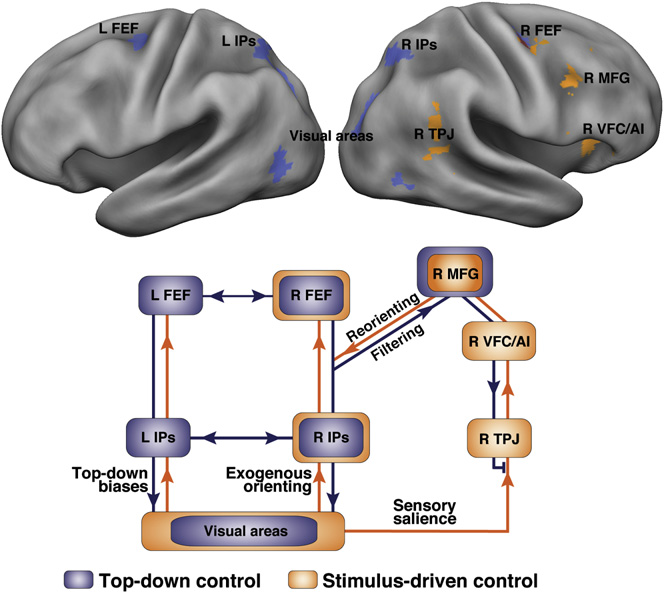
\includegraphics[scale=0.4]{img/attentionnetworks.png}
	\caption[Dorsal and ventral attention networks]
	{\small{Definition of dorsal and ventral networks from activation data and putative interactions. Taken from \textcite{corbetta2008reorienting}.}}
	\label{fig:Networks}
\end{figure}

A core part of the dorsal attention system are the FEF. In humans, the FEF is located in the rostral bank of a portion of the precentral sulcus at the caudal end of the middle frontal gyrus. It is primarily involved with transforming sensory signal into motor commands for intentional conjugate visual exploration to the contralateral visual space, and it is active in the disengagement from fixation that must precede each refixation saccade (\cite{goodwin2007cranial}; \cite{tehovnik2000eye}). Early insights about its function stem from stimulation studies with primates. Low-intensity electrical stimulation of the FEF in the bank of the arcuate sulcus in monkeys elicits saccadic eye movements directed contralateral to the stimulated hemisphere (\cite{tehovnik2000eye}; \textbf{Schall, 2009}). Work by \textcite{bruce1985primate} found that saccades elicited by stimulation at a particular region have a particular direction and amplitude that is independent of the orientation of the eyes. It further revealed a gradient of saccadic amplitudes from lateral to medial sites of the FEF: The more medially the stimulation of the primate arcuate sulcus, the larger the saccadic amplitude (\cite{bruce1985primate}). Hence, the ventrolateral portion of the FEF is generating shorter saccades, while the mediodorsal portion is generating longer saccades. This partialization of the FEF can be observed in its connectivity with other visual areas caudal to the central sulcus as well. The more ventrolateral portion of the FEF, responsible for generating shorter saccades, is - among other connections - interconnected with the perifoveal representation in retinotopically organized areas that represent central vision in the inferotemporal cortex. In contrast, the mediodorsal FEF, responsible for generating longer saccades, is interconnected with areas with a representation of the peripheral visual field, areas that emphasize peripheral vision or areas that are multimodal (\textbf{Schall, 2009}).
Stimulation studies in primates and high resolution fMRI experiments in humans further revealed that while the FEF is best known for its role in the generation of rapid saccadic gaze shifts, it also contains zones that are involved in the  control of other types of eye movements, among them pursuit, fixation, and vergence (changes of the depth of the gaze) eye movements (\cite{krauzlis2014eye}): Stimulation of the frontal pursuitzone in the fundus elicits pursuit eye movements directed ipsilateral to the stimulated hemisphere (Schall, 2009). The intracortical stimulation of several subareas within the FEF, among others a region within the pre-arcuate cortex in rhesus monkeys, immediately rostral to the saccade related anterior bank of the arcuate sulcus, triggers vergence movements, and shows an involvement in accomodation (Crosby et al., 1952, cited by \textcite{vernet2014corrigendum}). The FEF, therefore, seems to play a crucial role in all kinds of eye movements. \newline
However, as its involvement in the dorsal attention network suggests, the FEF is further involved in a number of aspects of higher cognition, such as attention, visual awareness, and perceptual modulation. The most compelling evidence stems from lesion studies: unilateral damage to the FEF results in contralateral neglect (\cite{crowne1981effects}). In healthy humans, \textcite{muggleton2003human} found rTMS at 10Hz for 500ms over the right FEF to impair only subtypes of visual search involving endogenous attention, namely where a visual target was neither salient nor predictable. Furthermore, activation in the FEF reflects deployment of attention even in the absence of accompanying eye movements to the region of interest, so called \textit{covert attention} (\cite{vossel2014dorsal}). \textcite{thompson2005visual} studied the FEFs role in target selection in primates performing a visual search task, finding evidence for the existence of a heatmap-like representation of saliency encoded in selective activation that is related to the overall behavioral relevance of visual stimuli, regardless of whether this relevance is derived from bottom-up stimulus properties or top-down knowledge and goals. This representation, the authors argue, arising from an integration of both top-down and bottom-up influences, then determines targets for foveation in the visual field in a 'the-winner-takes-it-all' fashion. 
As such, the involvement of the FEF in the various types of eye movements is modulated by the cognitive context (\cite{vernet2014corrigendum}). \newline
\textbf{TODO: THIS NEEDS A BETTER OUTRO}


\section{Movements of the eye}\label{section:eyemoves}
A central feature of the human retina is the fovea centralis, a specialised region about 1.5mm in diameter in the center of the retina (\cite{benninghof2004anat}). It serves only the central 1$^\circ$ of the visual field, but due to possessing the highest amount of cones of the retina, and an asymmetric distribution of ganglion cell density across the retina that advantages foveal information, it provides the greatest visual acuity (\cite{perry1986ganglion}). This asymmetry is propagated in the cortical representation of visual inputs from the retina. The magnification factor (MF), the linear extent of cortex devoted to each linear degree on the retina (\cite{daniel1961representation}), increases monotonically from periphal to foveal vision (\cite{daniel1961representation}). As a result, in almost all visual brain areas, both cortically and subcortically, the fovea has the greatest representation, and full visual acuity can therefore only occur at the fovea. 
Due to this constraint, humans need the ability to, first, align the fovea rapidly to an object of interest and, second, keep the fovea aligned to it for a sufficient amount of time in order to maximize the efficiency of foveal vision and perceive objects of interest in greatest detail. An exploration of a visual scene is hence performed in a stepwise manner and requires the described sequence of eye movements to sequentially explore all areas of interest. To accomplish this, the human eye is capable of a number of different eye movements. In its most simple form, the sequence consists of rapid saccadic eye-movements, redirecting the fovea from one object of interest to the next, followed by phases of \textit{fixation} that keep the fovea aligned for visual analysis. As saccades reach speeds of up to 500 $^\circ$/sec, small, corrective post-saccadic oscillations, so called \textit{glissades}, correct minor deviations of saccade target and actual saccade endpoint. Additionally, \textit{smooth pursuits} enable a viewer to track moving objects, while \textit{vergence} movements are necessary for accommodating different depths (\cite{holmqvist2011eye}). The following table \ref{table:eyemovements} provides an overview of these movements and their characteristics. Note, however, that most work on eye movements was conducted on static stimuli, and eye movements on moving images could possess differential characteristics. \textcite{dorr2010variability} for example investigated fixation characteristics differentially for varying stimuli and found Hollywood movies to elicit longer fixations (mean: 354ms, median: 253ms) than static images. \newline
  
\begin{table}[H]
	\begin{center}
		\begin{tabular}{lC{3cm}C{3cm}C{3cm}}
			\thickhline 
			\textbf{Type}	& \textbf{Duration(ms)} & \textbf{Amplitude (degrees)} & \textbf{Velocity ($^\circ$/sec)} \\ \hline
			Fixation 		& 200-300  & -  &  - \\
			Saccade 		& 30-80   & 4-20  & 30-500 \\
			Glissade			& 10-40   & 0.5-2  & 20-140 \\
			Smooth pursuit			& -  & -  &  10-30 \\ \thickhline
		\end{tabular}
		\caption[Movements of the eye]{\small{An overview of major types of eye movements and their characteristics, taken from \textcite{holmqvist2011eye}.}}
		\label{table:eyemovements}
	\end{center}
\end{table}

With regard to the scope of this thesis, and as eminent from the fundamental principles of foveal vision, saccades are the type of eye movement of particular relevance to the study of visuospatial attention (\cite{kowler2011eye}). Saccadic eye movements are controlled by a number of highly interconnected brain region, both cortical and subcortical (\cite{munoz2002commentary}, see figure \ref{fig:saccregions}), but in the cortex, the FEF are seen as the principal region involved in oculomotor control (\cite{leichnetz1988higher}). The FEFs further involvement in visuospatial attentional processes emphasizes its role as a site of conversion for the selection of visual targets for saccades and visuospatial attention (\cite{corbetta2002control}; \cite{kowler2011eye}). Thus, in regard to the study of visuopatial attention and eye movement they appear as an ideal subject of interest.




\begin{figure}
	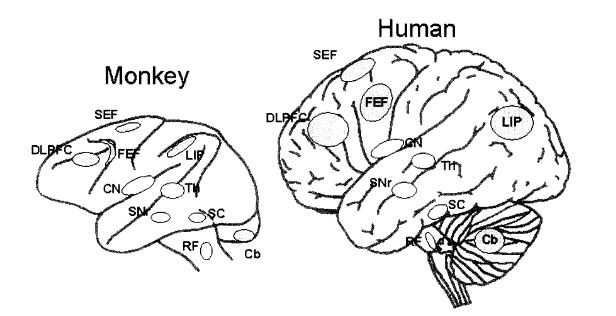
\includegraphics[scale=0.5]{img/saccregions.png}
	\caption[Regions involved in saccadic eye movements]{\small{Brain areas involved in the control of saccadic eye movements in monkey (left) and human. \textit{Cb}: Cerebellum, CN: Caudate nucleus, \textit{DLPFC}: dorsolateral prefrontal cortex, \textit{FEF}: Frontal eye field, \textit{LIP}: Lateral intraparietal area; \textit{RF}: Reticular formation, \textit{SC}: superior colliculus, \textit{SEF}: supplementary eye field, \textit{Snr}: substantia nigra pars reticularis, \textit{Th}: Thalamus. (Taken from \textcite{munoz2002commentary})}}
	\label{fig:saccregions}
\end{figure}

\section{Insights on function and location from naturalistic stimulation}\label{section:shortcomings}
Visuospatial attention is usually studied by means of highly controlled experimental tasks, such as Posners' cueing paradigm (\cite{posner1980attention}) or simple visual search tasks. While well controllable, these conventional laboratory experiments suffer from a lack of ecological validity and fail to evoke realistic competing demands for visuospatial attention. As \textcite{hasson2004intersubject} noted, controlled experimental settings bear little resemblance to natural viewing for at least four reasons: 1) Lack of complex visual scenes (i.e. presentation of visual stimuli in isolation), 2) Lack of (complex) movement, 3) Lack of unconstrained eye movement, and 4) Lack of interactions between vision and additional modalities, context and emotional valence. Naturalistic stimulation such as watching movie clips, in contrast, does not suffer from these shortcomings and, as \textcite{hasson2010reliability} showed, does also not lack experimental control. During the past decade, therefore, while static images have been an object of interest in the analysis of gaze distribution and attention from the early works of \textcite{yarbus1967eye} onwards, movies or videos became a promising stimulus choice as well. They contain interesting, multisensory stimuli and are more representative of natural vision arrays than static pictures. As movie content constantly changes and includes both salient elements such as motion, as well as top-down components from the attempts to comprehend and interpret the content (\cite{ross2013eye}) movies represent an ideal possibility to study the dynamic and complex interplay of attentional processes ecologically valid   (e.g. in \textcite{hasson2004intersubject}; \cite{carmi2006visual}; \cite{tseng2009quantifying}; \cite{dorr2010variability}). \newline
Localization of areas such as the FEF in turn is most reliably conducted via micro-stimulation in animals. Localization through non-invasive methods in humans is more challenging, but studies employing positron emission tomography (PET) (e.g. \textcite{paus1996location}, \cite{kawashima1998oculomotor}), magneto-encephalography (MEG) (e.g. \cite{ioannides2004meg}), fMRI (e.g. \cite{petit1999functional}; \cite{connolly2002human}), and transcranial magnetic stimulation (TMS) (see \textcite{vernet2014corrigendum}, for an overview) were able to shed light on the possible location of the FEF in humans. The methods for FEF localization are usually behavioral paradigms with either general oculomotor tasks (\cite{paus1996location}), or more specific oculomotor task such as instructed fixations, pro- and antisaccades (\cite{connolly2002human}) or tracking of horizontal step stimuli (\cite{alkan2011differentiation}). However, an overall view of this literature also reveals the large variability of reported localizations between studies (see e.g. \textcite{paus1996location}; \textcite{vernet2014corrigendum}, for overviews), and there is no consensus on whether these discrepancies arise from methodological differences in the choice of imaging technique or behavioral paradigm, or inter-individual differences between participants.  Also, while capable of localizing areas undoubtedly involved in the movement of the eyes, the displayed movements are not performed under unconstrained conditions and it remains unknown whether uncontrolled eye movements under naturalistic viewing behavior can be capable of providing similar location information as well, if not even additional information when taking cognitive context such as attention deployment into account.\newline
The present thesis aims to fill this gap in the literature by means of fMRI and eye tracking data during naturalistic stimulation. Due to its ready availability coming from the Psychoinformatics Lab itself, its incredible data richness, and its employment of naturalistic stimuli in form of a Hollywood movie, the studyforrest datasets were selected as the data basis of the analysis.

\section{Utilizing eye movements in the study of attentional deployment}\label{section:eyeutils}

In order to study visuospatial attention, a quantitative measure of attentional deployment was derived using eye gaze information in the form of \textit{scanpaths}.
The term scanpath refers to the trace of eye-movements in space and time (\cite{holmqvist2011eye}). In its most simple form, it is formed by a succession of fixations and saccades that define the particular sequence in which the eyes explore a visual scene (\cite{anderson2015comparison}). As opposed to other measures that summarize eye gaze, such as heatmaps, and as  emphasized by \textcite{holmqvist2011eye}, the order of eye-movements is relevant - a different order of elements in the representational sequence of eye-movements constitutes a different scanpath. \newline
The analysis of scanpaths has been used for decades to gain insights into the viewers’ mental processes, especially those concerning visuo-spatial attention. \textcite{yarbus1967eye} wrote: 

\begin{quotation}
\footnotesize{„Eye-movements reflect the human thought processes; so the observer‘s thoughts may be followed to some extent from records of eye-movements (the thought accompanying the examination of the particular object). It is easy to determine from these records which elements attract the observer‘s eye (and, consequently, his thought), in what order, and how often“.}
\end{quotation}

Following this reasoning, the comparison of scanpaths of different subjects constitutes a measure of similarity in the different subjects’ attentional processes and adds a useful dimension to the traditional analysis of eye-tracking data. In recent years, many approaches for scanpath comparisons were developed and implemented in various software solutions. Among them are methods based on (semantic) areas of interest (AOIs) such as the \textit{Levenshtein distance} (\cite{levenshtein1966binary}), or an improved generalization of it in \textit{ScanMatch} (\cite{cristino2010scanmatch}), methods based on attention maps such as \textit{AMAP} (\cite{ouerhani2004empirical}), methods employing machine learning algorithms such as \textit{SMAC with HMM} (\cite{coutrot2018scanpath}), or methods based on vector-geometry such as \textit{MultiMatch} (\cite{jarodzka2010vector}). The latter method has been developed specifically to overcome known shortcomings of many previous methods that limit their informative value, stemming from a loss of information due to the use of coarse aggregate measures of eye movement, susceptibility of the results of a comparison to influential data points due to arbitrary classifications, or both. The method does not rely on AOIs and hence achieves a finer level of detail in scanpath comparison. It takes temporal order, location in space, durations of fixations, and the shape of eye-movements into account, and is thus a comprehensive evaluation of multiple scanpath characteristics. In evaluations with simulated and actual eye-tracking data, the method was found to be robust against spatial noise, sensitive to position, order and fixation duration, and outperformed the ScanMatch method in AOI border cases (\cite{dewhurst2012depends}). In a comprehensive test of eleven common scanpath comparison methods on static real-life photographies, MultiMatch was found to be robust in general, however with high differences in the duration measure depending on the viewing time for the stimuli (\cite{anderson2015comparison}). As it additionally was successfully used to study mental activity involved in perceiving visual input by others (\cite{french2017evaluation}) already, the MultiMatch method was chosen to be employed in the current thesis to derive a measure for attentional processes of participants during movie watching. 
The original implementation, however, only existed as a Matlab toolbox shared upon request by the corresponding author of the respective publication (\cite{dewhurst2012depends}). This reliance on closed-source software and barriers in retrieval of the software\footnote{While acquisition of the toolbox via e-mail was prompt and complication-free, later correspondence with several of the authors was an odyssey of expired email addresses, changed affiliations and digital communication allegedly lost in the void of the Internet.} hinder the wider usage and potential improvement of the method. A publicly available, open-source implementation however would instead facilitate scientific work. Therefore, the method was ported from Matlab into Python and transformed into the pip-installable module multimatch\footnote{The module can be install via ```pip install multimatch```. A corresponding publication (Wagner \& Hanke) in the Journal of Open Source Software (JOSS) in currently under review. The sourcecode can be found at github.com/AdinaWagner/multimatch}. An overview of the method is available in section \ref{section:multimatch}

\section{Investigating functional specificity with functional sensitivity profiles}\label{section:methodintroduction}

The general approach of localization consists of contrasting experimental conditions known to activate specific functional regions in a general linear model (GLM), for example the contrast between activation during static images of houses and static images of faces to localize the FFA (\cite{fox2009defining}), or the use of instructed horizontal saccades versus fixations to localize the FEF (\cite{connolly2002human}). This approach suffers from a number of drawbacks: \newline
First, as outlined in \ref{section:shortcomings}, the employed artificial stimulation is not ecologically valid, which decreases the sensitivity of functional localizers and thus their applicability across studies. Secondly, a reliance on narrow stimulus categories and simple contrasts omits insights into further stimulus aspects of potential relevance - especially since an exact contrast between conditions accounting for various ROI-specific factors is not known ahead of time, and thus cannot be incorporated into the localizer GLM contrast. Moreover, it is challenging to differentiate functionally related but different ROIs with a simplistic experimental design. Therefore, localization often further requires to take spatial information for functionally close regions (such as OFA, FFA) into account.
Lastly, changes in statistical thresholds can alter localization results substantially (\cite{fox2009defining}) and introduce an additional source of \textit{researchers degrees of freedom} into an analysis.\newline
The approach outlined in this section is designed to estimate a maximally discriminative contrast between the functional signatures, i.e. the activation time courses, of any two ROIs in question, and to use the available experimental design - regardless of complexity - to provide a functional description for it.\newline
The method relies on sensitivity profiles derived during a classification analysis. Two different algorithms for classification were investigated, and will be introduced in the next section. In order to validate the method, its applicability and generalization capabilities were first tested on a general localization paradigm, and later movie-data, for already localized ROIs, which will be elaborated on in section \ref{section:methodvalidation}.



\subsection{Gaussian Naive Bayes classifier}
Machine learning refers to the study and construction of software that can learn from data without being explicitly programmed. Especially in the data-rich environment of neuroimaging, machine learning algorithms and techniques have gained immensely in popularity and significance as for their ability to detect hidden patterns and trends in the data (Vogt, 2018). One particular type of tool from machine learning is a so called \textit{classifier}. A classifier is trained on a subset of data, the \textit{training set}, and is then used for predictions on a previously unseen subset of data, the \textit{test set} (Nguyen \& Zeigermann, 2018). \newline
More formally, a classifier is a function created from training data to predict the value of a class attribute $C \in \{1, \ldots, r\}$ (the \textit{label}), given the predictive \textit{features} $X = (X_1, \ldots, X_d)$ of an unseen instance $x = (X_1, \ldots, x_d)$. Suppose $(X, C)$ is a random vector with a joint feature-label probability distribution $p(x, c)$. A classifier $\psi$ is the function that maps X into C:

\begin{equation}\label{classifier}
\psi: \{1, ... r_1\} \times  \ldots \times \{1, ..., r_d\} \rightarrow \{1, ..., r\}
\end{equation}
\begin{equation}
x \mapsto c,
\end{equation}

and is learned from a training set $S_n =\{(x^{(1)}, c^{(1)}), \ldots, (x^{(n)}, c^{(n)}) \}$ with a certain classifier algorithm A($\cdot$).
\newline
The overall aim of the classification analysis in this thesis was to derive a sensitivity measure in the form of feature weights. There are a number of different classification algorithms available to build classification models, and based on prior work of \textbf{Nastase et al. (2016)}, a \textit{linear Gaussian Naive Bayes} classifier (GNB) showing high classification accuracy and easy interpretability was further explored in this thesis. \newline
The algorithm belongs to the family of Naive Bayes algorithms which use a probabilistic approach to classification, utilizing the Bayes theorem to capture the relationships within input data and output label. Given some samples $x_1, \ldots, x_n$ with a number of characteristics on different features, and labels $c_1, \ldots, c_r$, naive Bayes classifier learn a model of the joint probability, $p(x, c)$, and make predictions by using Bayes theorem to calculate the probability of a label, given the feature characteristics of a sample, $p(c|x)$. Two fundamental assumptions exist for these algorithms. \newline 
\begin{itemize}
	\item \textit{Conditional independence}: Each feature $x_i$ is independent of every other feature $x_j$ for $j \neq i$ given the outcome $c_r$.
	\item \textit{Equal contribution of features}:  Each feature is given the same weight for the outcome prediction. 
\end{itemize} 
A linear Gaussian Naive Bayes classifier further assumes the data to be distributed according to a Gaussian distribution, and it assumes the feature variance to be independent of class (i.e. $\sigma_{i, 0}^2 = \sigma_{i, 1}^2$). Given the latter assumption holds, the decision boundery between any two classes 1 and 0,
\begin{equation}
\prod_{i=1}^{d} P(X_i |C = 0)P(C=0) = \prod_{i=1}^{d} P(X_i |C = 1)P(C=1),
\end{equation}
is linear (for the mathematical proof, see e.g. \textcite{DBLP:books/daglib/0087929}), chapter 3). The feature weights of this classifier are defined as
\begin{equation}
w_i = \sum_{i}\frac{\mu_{i, 0}-\mu_{i, 1}}{\sigma_{i}^{2}}.
\end{equation}


\subsection{A 'transposed' approach to classification}
The method presented here follows and extends work by \textbf{Nastase et al. (2016)}: Following a classification of voxels (samples) to ROIs (labels) based on the observed data in the ROIs from other participants, a subsequent analysis of the classifiers sensitivity profile obtained from a decision between ROI pairs is used to shed light onto their functional distinctiveness. As opposed to the common approaches at classification in neuroimaging, the datasets are transposed: The features in this classification problem are time points, while voxels constitute samples. \newline
In a first analysis step, a sensitivity profile of two ROIs is obtained via classification analysis. As the dataset is transposed to have time points as features, this sensitivity profile is a time course of sensitivities: each weight corresponded to the difference in mean activation of all voxels given the label (ROI) at one time point, normalized by their common variance. In an examplary decision between ROIs A and B, a negative weight corresponds to an overall higher activation in B at this particular point in time. In a second step, this time course is entered as a criterion in a GLM with details about the experimental design at different time points as regressors. The resulting coefficients indicate the importance for each regressor (i.e. stimulus characteristic) for the distinction between ROIs.\newline
[HOW CAN WE USE THIS FOR FEF]


\chapter{Methods}\label{section:methods}

The following method section attempts to give a concise description of this thesis' data basis, fMRI and eye-tracking, and the employed and developed methods, MultiMatch and sensitivity analysis. 

\section{Data basis}

Data stems from the 2016 released extension of the studyforrest dataset (\cite{hanke2016studyforrest}; \cite{sengupta2016studyforrest}; all data and code publicly available at https://github.com/psycho-informatics-de/studyforrest-data-phase2). In this extension, $N = 15$ right-handed participants (age range 21 – 39 years, mean age 29.4 years, six female, normal or corrected-to-normal vision), who had previously participated in the studyforrest project, watched the audio-visual movie “Forrest Gump” (R. Zemeckis, Paramount Pictures, 1994) during simultaneous fMRI and eye-tracking recording, and underwent a traditional localizer paradigm for higher visual areas: The fusiform face area (FFA), the occipital face area (OFA), the extrastriate body area (EBA), the hippocampal place area (PPA), the lateral occipital complex (LOC) and early visual cortex (\cite{sengupta2016studyforrest}).

\subsection{Stimulus material}

Stimulus material for the audiovisual movie was the German dubbed version of Forrest Gump, overlaid with a German audio-description (Koop, Michalski, Beckmann, Meinhardt \& Benecke, produced by Bayrischer Rundfunk, 2009), originally broadcast as an additional audio track for visually impaired recipients on Swiss public television. The additional audio track consists of a male narrator describing the visual content of a scene between dialogs, off-screen-speech or any other relevant audio-content of the movie (\cite{hanke2014high}). The video track for the movie stimulus was re-encoded from Blu-ray into H.264 video (1280 x 720 at 25 frames per second (fps)). In accordance to the procedure in an earlier phase of the studyforrest project, the movie was shortened by removing a few scenes less relevant for the major plot to keep the fMRI recording session under two hours. The shortened movie was then segmented into eight segments of roughly the 15 minutes of length (for an overview on segment duration, final stimulus content and detailed procedures see \textcite{hanke2014high}). Stimulus material for the localizer paradigm consisted of 24 unique grayscale images for each of six different categories (faces, bodies, houses, scenes, everyday objects, and scrambled images) at a resolution of 400x400px, matched in luminance, and displayed at 10x10$^\circ$ of visual angle (\cite{sengupta2016studyforrest}).


\subsection{Procedures}
Functional MRI data acquisition for the audio visual movie was undertaken in two consecutive recording sessions on the same day, with a break of flexible duration. Within each session, four movie segments were presented in chronological order (\cite{hanke2016studyforrest}).  Prior to each segment an eye-tracker calibration with a 13-point sequence and accuracy validation was performed.
Segments were succeeded by another accuracy validation and participants were asked to rate their experience (“How deeply did you get into the story?”) on a scale from 1 (not at all) to 4 (a lot). Visual stimuli were projected on to a screen inside the bore of the magnet using an LCD projector, and presented to the subjects thought a front-reflective mirror on top of the head
coil at a viewing distance of 63cm. The screen dimensions were 26.5cm x 21.2cm at a resolution of 1280 x 1024 px with a 60Hz video refresh rate (\cite{sengupta2016studyforrest}). Eye-tracking was performed with an Eyelink 1000 (software version 4.594) using monocular corneal reflection and pupil tracking with a temporal resolution of eye gaze recordings of 1000Hz. The camera was mounted at an approximate distance of 100cm to the left eye of subjects, which was illuminated
by an infrared light source (\cite{hanke2016studyforrest}). Movie presentation and eye-tracking were synchronized by starting the eye gaze recording as soon as the stimulus computer received the first fMRI trigger signal. Timings of subsequent trigger pulses and onsets of every movie frame
were logged. Using a 3 Tesla Philips Achieve dStream MRI scanner with a 32 channel head coil, T2*-weighted echo-planar images (gradient-echo, TR = 2s, echo time = 30ms, flip angle = 90) were acquired during movie watching. For the eight segments, 451, 441, 438, 488, 462, 439, 542, and 338 volumes were acquired, respectively (\cite{hanke2016studyforrest}).\newline

In the localizer paradigm, participants viewed the different object categories in a total of four block-design runs, with two 16s blocks per stimulus category. The order of the individual images per category differed across runs and participants, but the sequence of category blocks was the same for every run and participant. Localizers for higher visual areas (FFA, OFA, PPA, LOC, EBA, and early visual cortex) were obtained by the original authers of the studyforrest extension by means of the two-level GLM analysis on contrasts of activation between objectcategories (for details, see \cite{sengupta2016studyforrest}).

\subsection{Data Analysis}
Data preprocessing and analysis were conducted with a multitude of Python-based software packages. Preprocessing of data relied primarily on custom made workflows written with nipype (\cite{gorgolewski_krzysztof}), and utilizing FSL (\cite{jenkinson2012fsl}). Much of the data analysis was done using pyMVPA (\cite{hanke2009pymvpa}). Datalad, a version control tool for scientific data (https://zenodo.org/record/1470735), served as a backbone for all own work presented in this thesis. If applicable and unless otherwise stated, the alpha level for statistical significance was set to $\alpha = 0.05$.

\subsection{Preprocessing}
Eye-tracking data were normalized such that all gaze coordinates are in native movie frame pixels, with the top-left corner of the movie frame located at (0, 0) and the lower-right corner located at (1280, 546) (\cite{hanke2016studyforrest}). The amount of unusable data, primarily due to signal loss due to eye blinks, ranged from less than 1 to 15\% for 13 of the 15 in-scanner subjects (the other two subjects’ data contained 85 and 36\% of data loss, respectively). In-scanner acquisition had an approximate spatial uncertainty of 40px according to the calibration procedure. \newline
The raw eye tracking data was classified into different eye movements. For this, based on an adaptive, velocity-based algorithm proposed by \textcite{nystrom2010adaptive}, Dar, Wagner and  Hanke (in preparation) implemented a data-driven algorithm for robust eye movement detection for natural viewing (REMoDNaV) in Python, independent of this thesis\footnote{The sourcecode can be found at github.com/psychoinformatics-de/remodnav}. All results of this algorithm are publicly available at [\textbf{TODO: }URL here]. The algorithm categorizes the raw data into the eye movement categories saccades, fixations, post-saccadic oscillations (glissades), and disregards any unclassifiable data (such as blinks). The eye events are reported together with their start- and end coordinates, their onsets and duration in seconds, their velocity and the average pupil size.

Motion-corrected fMRI data in a study-specific group-template were obtained from the respective Github repositories via datalad [CITE]. In a first step, both datasets, localizer and movie-data, were preprocessed identically using a custom made nipype workflow, consisting of whole-brain masking, high-pass filtering and smoothing with a Gaussian kernel of 4mm FWHM\footnote{All code for preprocessing and analysis can be found at https://github.com/AdinaWagner/localizer}. \newline

\subsection{Extraction and processing of eye tracking data}

For the extraction of saccadic eye events, the results where filtered to include only saccades. For the computation of event files following the BIDS standard (\cite{gorgolewski2016brain}), the Cartesian coordinates of the saccades were transformed into Polar coordinates (angle and length). Based on their angle, saccades were classed into event types describing eight different orientations in the visual field. Saccade onsets and durations were extracted from the REMoDNaV output. The resulting event file per run hence contained the onset, duration, amplitude (length) and direction of saccades. \newline


\section{MultiMatch}\label{section:multimatch}
For the purpose of this thesis, the MultiMatch method for scanpath comparison (\cite{jarodzka2010vector}) was ported into Python for further use on the preprocessed eye movement data. An overview in pseudocode is outlined in algorithm \ref{algo:multimatch}. \newline 
The method takes two n x 3 fixation vectors of two scanpaths with x-coordinates, y-coordinates, and duration of fixations as columns as its input. Based on the coordinates and durations of fixations, the scanpaths are represented as geometric vector sequences as shown in figure \ref{fig:Polar_to_cartesian}:

\begin{figure}[H]
		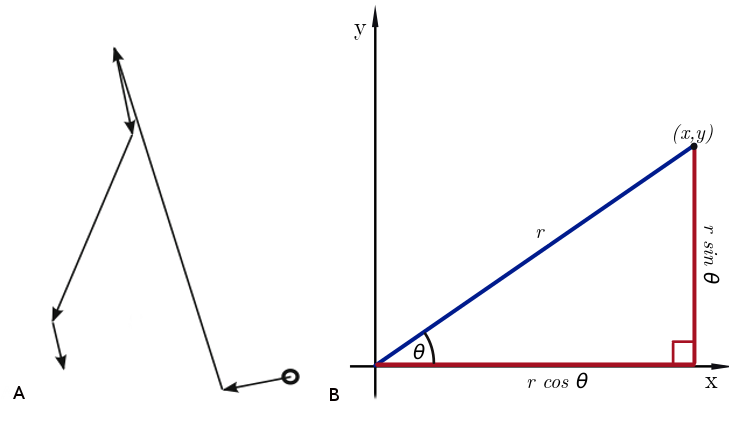
\includegraphics[scale=0.35]{img/scanpathconversion.png}
		\caption[Geometric representation of eye movements]
		{\small{\textit{A: Geometric scanpath representation.} An idealized saccade is represented as the shortest distance between two fixations. The Cartesian coordinates (x, y) of the fixations are thus the starting and ending points of a saccade. The length of a saccade in x (or y) direction is computed as the difference in x (or y) coordinates of starting and ending point. \newline
		\textit{B: Length and angle computation.} Length from the coordinate origin, rho, is computed as the Euclidean norm by means of the Pythagorean theorem: $r = \sqrt{ x^2 + y^2}$. The angle in radians, theta, is computed as a variation of the arctangent function as the angle from positive x axis to the point (x, y), with positive values denoting counterclockwise angle from positive x axis and negative values denoting clockwise angles: $\theta = arctan2(x, y)$.}}
		\label{fig:Polar_to_cartesian}
\end{figure}

To reduce complexity, the scanpaths are simplified according to angle and amplitude in an iterative procedure. Two or more saccades are grouped together if angles between two consecutive saccades are below an angular threshold \textit{TDir}, or if the amplitude of successive saccades is below a length threshold \textit{TAmp}, as long as intermediate fixations of the saccades are shorter than a duration threshold, \textit{TDur}. As such, small, locally contained saccades, and saccades in the same general direction are summed to form larger, less complex saccades. \newline
In order to find pairings of saccade vectors to compare, the simplified scanpaths are temporally aligned. The aim is to not necessarily align two saccade vectors that constitute the same component in  their respective vector sequence, but those two vectors that are the most similar while still preserving temporal order. In this way, a stray saccade in one of the two scanpaths does not lead to an overall low similarity rating, and it is further possible to compare scanpaths of unequal length.  To do so, all possible pairings of saccades are evaluated in similarity by the vector differences between all pairings (shape): The vector differences between each element $i$ in scanpath $S1 = {u_1, u_2, \ldots, u_m}$ and each element $j$ in scanpath $S2 = {v_1, v_2, \ldots, v_n}$ are computed an stored in a Matrix $M$ as weights that denote similarity, with low weights corresponding to high similarity. In a next step, an adjacency matrix is build, defining the rules on which connection between matrix elements are allowed to preserve the temporal order of saccades. Together, matrices M and the adjacency matrix constitute a matrix representation of a directed, weighted graph (\ref{fig:directedgraph}). Elements of the matrix are nodes, the connection rules constitute edges and the weights define the cost associated with each connection. 
In the generic example in figure \ref{fig:directedgraph} the edge between node (1, 1) and node (1, 2) has an associated weight, or cost, of $w_2$. 


\begin{figure}
	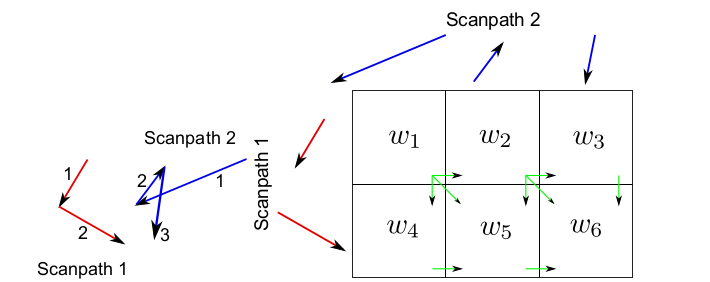
\includegraphics[scale=0.4]{img/weightedgraph.png}
	\caption[Scanpath alignment as a shortest-path-problem]
	{\small{The elements of two hypothetical scanpaths (left) are used to compute vector differences between all possible pairings as weights $w_1, \ldots, w_6$ in a Matrix $M$ (right). Green arrows indicate connection rules defined by an adjacency matrix. Taken from \textcite{jarodzka2010vector}}}
	\label{fig:directedgraph}
\end{figure}

A Dijkstra algorithm (\cite{dijkstra1959note}) is used to find the shortest path from the top left node, the first two saccade vectors, to the bottom right node, the last two saccade vectors. “Shortest” path is defined as the connection between nodes with the lowest possible sum of weights. The path returned by the Dijkstra algorithm is a sequence of indexes, denoting pairings of saccade vectors from each scanpath, and as such the desired alignment of scanpaths (\cite{dewhurst2012depends}).  Finally, in a last step, five measures of scanpath similarity (see figure \ref{fig:simmeasures}) are computed for a multidimensional similarity evaluation. This is done by performing simple vector arithmetic on all aligned saccade pairs $(u_i, v_j)$, normalizing the results according to a certain metric, and taking the median of the results. All five measures are in range [0; 1] with higher values indicating higher similarity between scanpaths on the given dimension. \newline

\begin{figure}[H]
	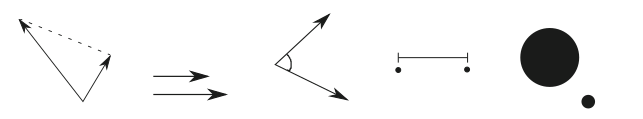
\includegraphics[scale=0.5]{img/simmeasures.png}
	\caption[Similarity measures]{\small{\textbf{Shape}: Vector difference between aligned scanpaths, normalised by 2x the screen diagonal. \textbf{Length}: Difference in vector lengths, normalized by the screen diagonal. \textbf{Angle}: Angular distance between saccade vectors, normalized by $\pi$. \textbf{Position}: Position difference of fixation, normalized by the screen diagonal. \textbf{Duration}: Duration differences of aligned fixations, normalized against maximum duration within the comparison.}}
	\label{fig:simmeasures}
\end{figure}


\begin{algorithm}
	\begin{small}
	\SetKwInOut{Input}{Input}
	\SetKwInOut{Output}{Output}
	
	\Input{nx3 fixation vectors (x, y, duration), simplification thresholds $T_{Amp}$, $T_{Dir}$, $T_{Dur}$}
	\Output{eventfile: onset of scanpath, duration, and five similarity measures range [0;1]}
	\For{each fixvector}
	{ 
		\For{fix in fixvector}
		{
			fixation\_x, fixation\_y, fixation\_dur = $x, y, duration$ \;
			saccade\_x(y) = fixation\_x(y)$_{fix}$ $-$ fixation\_x(y)$_{fix+1}$ \;
			saccade\_lenx(leny) = fixation\_x(y) $-$ saccade\_x(y)\;
			saccade\_rho, saccade\_theta = cartesian2polar(saccade\_lenx, saccade\_leny) \;
			\textbf{eyedata} = [fixation\_x, fixation\_y, fixation\_dur, saccade\_x, saccade\_y, \newline saccade\_lenx, saccade\_leny, saccade\_rho, saccade\_theta]
		}
		\While{simplification is still possible}{
			\If{angle(saccade$_{i}$, saccade$_{i+1}) < TDir$ \bfseries{and} $fixation\_dur < TDur$}
			{combine saccades}
			\If{saccade\_rho$_i$, saccade\_rho$_{i+1}$) < TAmp \textbf{and} fixation\_dur $<$ TDur}{combine saccades}
		}
		\For{pair of (simplified) scanpaths $S1 = \{u_1, \ldots, u_m\}, S2 = \{v_1, \ldots, v_n\}$}
		{
			calculate M: Matrix of saccadelength differences between each $i \in S1$ and  $j \in S2$\;
			create a directed graph with elements of M as weights $w_1, \ldots, w_i$\;
			align scanpaths with $min(\sum w)$ from $M(0,0)$ to $M(n,m)$ via Dijkstra algorithm\;
		}
		\For{pair($u_i,v_i$) in aligned scanpaths}
		{
			angular difference = angle($u_i, v_1$)\;
			position difference = $\sqrt{(x(u_i) - x(v_i))^2 + (y(u_i) - y(v_i))^2}$ \;
			vector difference = $\sqrt{(len\_x(u_i) - len\_x(v_i))^2 + (len\_y(u_i) - len\_y(v_i))^2}$\;
			length difference = $abs(rho(u_i) - rho(v_i))$\;
			duration difference = $abs(dur(u_i)-dur(v_i))$ \;
		}
		normalize angular difference by $\pi$\;
		normalize vector difference by 2x the screen diagonal (maximum theoretical distance)\;
		normalize length difference by the screen diagonal\;
		normalize position difference by the screen diagonal\;
		normalize duration difference by maximal duration difference in the scanpaths\;
		\textbf{return} median for each similarity measure
	}
	return \textbf{similarity measures}
	\caption{The MultiMatch Algorithm}
	\label{algo:multimatch}
\end{small}
\end{algorithm}

\subsection{MultiMatch and the studyforrest dataset: multimatch\_forrest}
The extraction and processing of eye events for further use with multimatch to estimate a measure of exogenous attentional control included several considerations based on findings and known caveats in eye tracking and attention research with dynamic scenes. These considerations were implemented as additional functionality of the multimatch module to natively work with the studyforrest dataset as a data basis in the function \textit{multimatch\_forrest}. The additional functions are distributed along with the main algorithm in the multimatch module and are mainly concerned with automatic scanpath extraction from the approximately 15 minutes spanning and several eye-movement categories containing eye-tracking event files by user-defined rules. An overview in pseudocode can be found in algorithm \ref{algo:multimatch_forrest}. \newline
First, as the stimulus was dynamic, the start and end of pursuit movements were relabeled as fixations. This was done to accomodate the fact that most areas of interest in a movie are in motion, and what would be a fixation while viewing a static image would likely be a slow pursuit during movie watching. A different consideration concerned the selection of scanpaths from the approximately 15 minute long segments, as they are unsuitably long to derive a continuous attention measure or do a scanpath comparison on. It has been shown that subjects gazes have a bias towards the center in Hollywood movies (\cite{tseng2009quantifying}). This bias can at least in part be traced back to a strong center bias directly after cuts in dynamic scenes. \textcite{carmi2006visual} found the highest degree of exogenous attentional control (i.e. maximal inter-observer similarity in gaze as recorded via eye-tracking) in a moving collage of 50 heterogeneous video clips directly after cuts to new, semantically unrelated scenes. Without isolating cuts it therefore can not be disentangled whether the contribution of visual features of the movie on scanpaths stems from exogenous control from a movie element or from the sudden occurrence of a new scene after a cut. To not introduce such a confound in the eye-tracking data, the data was cut into shots that did not contain cuts to different scenes, relying on a location annotation by \textcite{hausler2016annotation}. The location annotation contained a detailed description of the timing of each of the 870 shots of the movie as well as information about the depicted location in different levels of abstraction. A shot is defined as a movie sequence between two cuts. In a first step, all consecutive short shots to the same locale (e.g. two consecutive, short movie shots in Forrest's bedroom, without any cuts containing semantically unrelated content) were grouped together. A “short” shot was defined as being shorter than the median length of 4.92s. This increased the median length of shots from 4.92s to 7.019s. These elongated shots are henceforth referred to as snippets. In a next step, within the scanpath comparison, the onset and offset times of the resulting snippets were extracted for every snippet longer than 4.92s. To not introduce an influence of snippet length into the similarity results, as longer movie snippets will be more likely to be less similar than short ones, scanpath lengths were standardized to approximately 4.92s seconds (the original median length). To further evade any problems associated with the center bias, scanpaths were extracted from the end of the snippet: The last oculomotor event within the range of the snippet marked the end of a scanpath. As such, scanpaths began maximally distant to the snippet onset.
As the eye movements of participants are interindividually different and don't correspond exactly to snippet timing, the precise onsets and resulting exact durations were computed as well, and stored for later use as regressors.

\begin{algorithm}[H]
	\begin{small}
	\SetKwInOut{Input}{Input}
	\SetKwInOut{Output}{Output}
	
	\Input{REMoDNaV eye movement datafiles per run, movie location annotation per run, desired length to elongate shots to \textit{ldur}, desired scanpath length \textit{dur}}
	\Output{One n x 3 fixation vector (x, y, duration) per shot > dur}
	{
		\If{$event_{row}$ == pursuit}
		{
			regard start and end points of pursuit as fixation
		}
	}
	\For{row in REMoDNaV datafile}
	{
		\If{$event_{row}$ == fixation}{
			extract x-, y-coordinate, duration}
		\If{x, y < 0 or x > 1280 or y < 720}{discard as out-of-bound gaze}
	}
	\For{row in annotation}
	{
		\If{($locale_{row} == locale_{row+1}$) and ($duration_{row}, duration_{row+1} < ldur$)}
		{combine to one shot}
	}
	\For{row in annotation}
	{
		\If{$duration_{row}$ > dur)}
		{extract shotonset and offset time}
	}
	\For{i in length(onset)}
	{fixvector$_i$ = REMoDNaV[REMoDNaV$_{onset} > onset_i$; REMoDNaV$_{onset}$ < offset$_i$]
	}
	return $\{$fixvector$_1$, \ldots, fixvector$_i$$\}$, onsets, durations
	\caption{The studyforrest specific functions of multimatch}
	\label{algo:multimatch_forrest}
	\end{small}
\end{algorithm}

\section{A novel approach for the analysis of ROI specificity}\label{newmethod}
This section outlines the proposed method in general, and provides examplary use cases in the form of two sequential validation analysis independent of the FEF localization. \newline
The general idea behind the proposed method is to derive a functional signature as a temporal course from two ROIs in question, and to explain the functional signature by providing a detailed description of the experimental design. This is realized with a two step procedure consisting of classification (1) and GLM analysis (2).\newline
The functional signature is obtained from a classifiers sensitivity profile in an n-fold leave-one-participant-out cross-validation: The classifier is trained on all subjects except for one and then tested on that out-of-sample individual, and this method was repeated for each of the subjects (step 1, classification analysis). Obtained sensitivity profiles per fold are averaged. The achieved overall classification accuracy serves as a measure of whether population wide functional specificity and sensitivity between the ROIs can be captured. In the second step (GLM), the averaged sensitivity profile is regressed onto the stimulus description for an estimate on how well the experimental design could describe ROI differences, and to point to the effects in the experimental design contributing to an ROI distinction as evident from the beta coefficients of the respective regressors. \newline
The classifier of choice, a Gaussian Naive Bayes classifier, was readily available in pyMVPA’s (\cite{hanke2009pymvpa}) mvpa2.suite python module as GNB() and customizable to be a linear classifier with the parameter \textit{common\_variance = True}. However, it lacked functionality to compute feature weights for a sensitivity analysis. Therefore, as a preliminary step, the GNB class in the sourcecode of the pymvpa package was extended and a subclass GNBWeights implemented. This made a sensitivity analysis possible, that returns the weights $w_i = \sum_{i}\frac{\mu_{i, 0}-\mu_{i, 1}}{\sigma_{i}^{2}}$ for each feature for any possible pair of labels in a binary decision. For an example, consider a classification task with three labels L0, L1, L2, and two features, F1, F2. The implemented sensitivity analyzer will for each possible pair of labels (L0 versus L1, L0 versus L2, L1 versus L2) return one weight per feature\footnote{The sourcecode for this change can currently be found in the following PR: https://github.com/PyMVPA/PyMVPA/pull/591/files}. \newline
As the dataset was transposed to have time points as features, each weight corresponded to the difference in mean activation of all voxels given the class at one time point, normalized by their common variance. In case of for example the decision between FFA and PPA, a negative weight therefore corresponds to an overall higher PPA activation at this particular point in time. The type of stimulation present at this point in the experimental design likely contributes to the distinction between the two areas, and the magnitude of its influence will be visible in its associated beta coefficient obtained from the GLM \newline
 

\subsection{Method validation}\label{section:methodvalidation}

In order to establish feasibility of the procedure and to test the generalization of the developed approach, the method was validated in a two-step procedure. As a sanity check, it was used on data from a common block design for ROI localization within the studyforrest dataset. As a measure of its capabilities to generalize to naturalistic stimulation, it was subsequently used with the studyforrests' movie data, collected on the same participants. For both datasets, six functional ROI masks (FFA, PPA, OFA, EBA, LOC, early visual cortex) were available to serve as labels during classification analysis. Both validating analyses were restricted to the FFA-PPA distinction as for the wealth of literature concerned with these ROIs. \newline
For use in the localizer dataset, the event files describing the stimulation protocol of the object-category task were used to compute a group-level event file. This was possible because the order of blocks was the same across runs and participants due to a coding error (see \cite{sengupta2016studyforrest}). For each participant, the onsets of each image were averaged. Deviations from individual onsets to the average group onsets were smaller than 0.5 seconds. Additionally, the first occurrence of an image within an object category was classed a new type of event with the suffix 'first', resulting in 12 regressors (face, face\_first, body, body\_first, house, house\_first, scene, scene\_first, object, object\_first, scramble, scramble\_first). This was done to account for any additional variation introduced by the change in categories. Using pyMVPAs fit\_event\_hrf\_model, the resulting events were entered as regressors to explain the time course of sensitivities. \newline
For generalization in the movie dataset, a stimulus description of the movie was obtained from two sources, the location annotation of \textcite{hausler2016annotation}, and an automatic facial feature extraction per frame of Hanke (unpublished, done using Google's Cloud Vision API via pliers (\textbf{McNamara et al. 2017})). An event was derived for each "setting" in the location annotation occurring more than once, for night-time, a scene being located exterior, general scene changes, and contextual jumps to future or past from the previous shot. The facial feature data was downsampled to 1 second and two conditions were derived, "face" for any 1 second time window with a maximum of less than 3 faces, and "many\_faces" for any 1 second time window with more faces present.

\section{TODO: FEF}
[this is a TODO]




\chapter{Results}

\section{Eye movements}
In order to check the validity of the eye-movement extraction with REMoDNaV, the mean and median duration of extracted fixations were compared to the results of \textcite{dorr2010variability}. Fixations as found by REMoDNaV had a length of mean = 0.326s, median = 0.256s, which corresponds closely to the aforementioned study's results (0.354s and 0.253s, respectively). Moreover, a comparison of algorithm performance and human coding in the spirit of \textcite{andersson2017one} by Dar, Wagner and Hanke (in preparation) showed the highest degree of concordance of all contemporary algorithms used in \textcite{anderson2015comparison}.

\bigskip

\section{Method validation}\ref{results_method}
Figure \ref{fig_locsens} shows the time course of sensitivities and the corresponding GLM fit. As visible both from the time series' appearance and the regression coefficients, stimulation with images of faces and, to a lesser extent, bodies, in particular the first of these stimuli per block, differentially activated FFA more than PPA. PPA in turn was differentially activated by stimulation with scenes.
\begin{figure}
	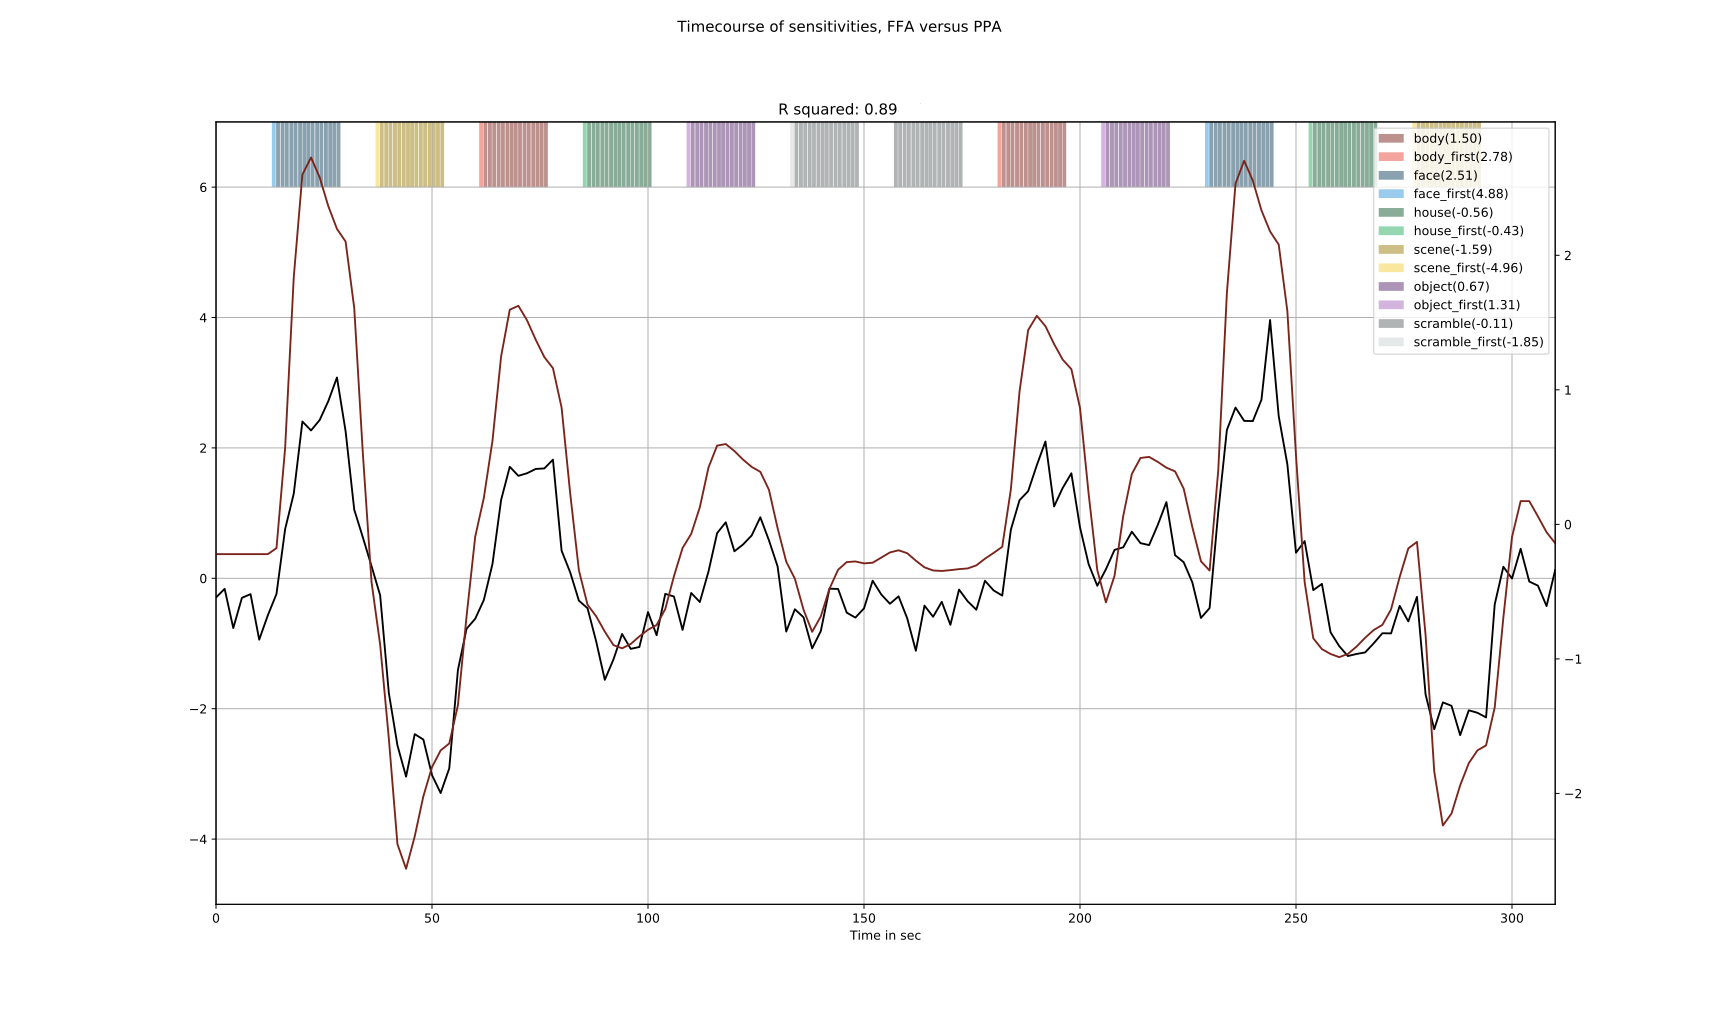
\includegraphics[scale=0.4]{img/res_sens_timecourse_localizer.png}
	\caption[Time course of sensitivites for localizer data]{\small{Black line: Sensitivities. Red line: GLM fit from regressing sensitivities onto the 12 event regressors derived from the object categories of the stimulation. Colors correspond to stimulation with one particular image type in time, beta values are given in brackets}}
	\label{fig:locsens}
\end{figure}
\section{Localization of the FEF}\label{results_FEF}

\chapter{TODO Discussion}\label{discussion}
maybe don't do summary section but place summary directly here.
\section{TODO Summary}
\begin{itemize}
	\item The aim of this thesis was to...
	\item Therefore, ... What did I do: MultiMatch, functional specifitity analysis
	\item The results show that...
\end{itemize}
\section{TODO Drawbacks and shortcomings}
\begin{itemize}
	\item A number of potential issues need to be addressed to access the validity of the results (maybe refer to Deborah Mayos Severe Testing ideas?)
	\item Attentional mode based on scanpath comparison: At best able to capture a measure of exogenous control? Give alternative explanation what might have been measured. Problem of 5 different similarity measures --- BUT successfully used by French et al., multidimensional construct preferable as might explain more variance (citation? check anderson or the other dewhurst publication) 
	\item Now trash all shortcomings and come to the conclusion that for was done and despite a number of limitations this thesis was able to advance the literature in the following ways
\end{itemize}
\section{TODO Conclusions}
\begin{itemize}
	\item now what have we all learned after reading this far?
\end{itemize}
\section{TODO Future directions}
\begin{itemize}
	\item further work on the ROI specificity to improve model fit
\end{itemize}


\chapter{Things that are still shitty}
\begin{itemize}
	\item too many passive constructions
	\item many long, incomprehensible sentences. boil it down to something simpler
	\item I need better verbal connections between sections. Short intros and outros of all main chapters.
	\item surely incomprehensible method description
	\item Citations are fucked up, take care of the bibtex style, its still according to macroeconomics, there has to be an example for APA on the internet somewhere
	\item all \textbf{bold} citations are not yet in bibtex, mostly because they are weird formats.
	\item prune references extensively after recent shortening spree (maybe simply disable nocite{*} if I'm lazy?)
\end{itemize}




\section{old examples as reminders}


\textbf{HOW TO DO A TABLE}
\begin{table}[H]
	\centering
		\begin{tabular}{lC{3cm}C{2cm}C{3cm}}
			\thickhline 
			\textbf{Variable}	& \textbf{Abbreviation} & \textbf{ADF} & \textbf{Significance}  \\ \hline
			Gross domestic product 	& GDP	& $-3.95$   & $p<0.05$  \\
			Industrial production	& IP	& $-4.13$   & $p<0.05$  \\			
			Private consumption		& PC	& $-3.26$   & $p<0.10$   \\			
			Unemployment rate  		& UR	& $-3.77$   & $p<0.05$  \\
			Consumer price index	& CPI	& $-3.65$ 	& $p<0.05$  \\
			Car sales volume		& CAR	& $-3.95$   & $p<0.05$  \\
			Interest rate			& IR	& $-3.33$   & $p<0.10$   \\ \thickhline
		\end{tabular} 
		\caption{Stationarity analysis for German macroeconomic variables (measured in relative changes)}
		\label{table:stationarity}
\end{table}

\textbf{HOW TO DO A NICE CORRELATION TABLE}
\begin{table}[H] 			
	\begin{center}
		\begin{tabular}{C{1.5cm}C{1.5cm}C{1.5cm}C{1.5cm}C{1.5cm}C{1.5cm}C{1.5cm}C{1.5cm}}
			\thickhline
			& \textbf{GDP} & \textbf{UR} 	 & \textbf{CPI}	   & \textbf{CAR}		& \textbf{PC}	 & \textbf{IP}	  & \textbf{IR}  	\\ \hline
			\textbf{GDP}	 & 	   & $-0.69$ & $0.35$  & $-0.54$ & $0.20$  & $0.98$  & $0.83$   \\ 
			\textbf{UR}	 & *** & 	 	 & $-0.58$ & $0.33$  & $-0.20$ & $-0.67$ & $-0.81$  \\ 
			\textbf{CPI}	 & **  & *** 	 & 		   & $-0.33$ & $-0.19$ & $0.39$  & $0.57$   \\ 
			\textbf{CAR}	 & *** & **      & **      & 	     & $0.35$  & $-0.58$ & $-0.42$ \\ 				
			\textbf{PC}	 &     &  	     &  	   &         &         & $0.09$  & $0.19$  \\ 
			\textbf{IP}	 & *** & *** 	 & ***	   & *** 	 &  	   & 	     & $0.79$  \\ 
			\textbf{IR}	 & *** & *** 	 & *** 	   & ***	 &  	   & *** 	 &   \\ \thickhline				
		\end{tabular}
	\end{center}
	\footnotesize Significance codes: *** $p<0.01$   ** $p<0.05$   * $p<0.10$. 
	Note: GDP=gross domestic product, UR=unemployment rate, CPI=consumer price index, CAR=car sales volume, PC=private consumption, IP=industrial production, IR=interest rate
	\begin{center}
		\caption{Correlations of German macroeconomic variables}
		\label{table:correlations}
	\end{center}
\end{table}	


\textbf{HOW TO DO SUBPLOTS}
\begin{figure}[H]
	\subfigure[German GDP growth rates]{\includegraphics[width=0.49\textwidth]{Plots/Plot_DE_GDP}}
	\subfigure[German industrial production growth rates]{\includegraphics[width=0.49\textwidth]{Plots/Plot_DE_IP}}
	\subfigure[German CPI growth rates]{\includegraphics[width=0.49\textwidth]{Plots/Plot_DE_CPI}}
	\subfigure[German private consumption growth]{\includegraphics[width=0.49\textwidth]{Plots/Plot_DE_PC}}
	\subfigure[German unemployment growth rates]{\includegraphics[width=0.49\textwidth]{Plots/Plot_DE_UR}}
	\subfigure[German car sales volumes growth rates]{\includegraphics[width=0.49\textwidth]{Plots/Plot_DE_Car}}
	\caption{German macroeconomic variables}
	\label{plot:macrovariables}
\end{figure}

\textbf{EQUATIONS AND SO FORTH}
\begin{equation}\label{MLR_eq}
y_i = \beta_0 + \beta_1 x_{1,i} + \ldots + \beta_k x_{k,i} + \varepsilon_i, \qquad i=1,\ldots, n
\end{equation}
for some real numbers $\beta_1, \ldots \beta_k$, where we denote the $i$-th observation of the dependent and the $j$-th predictor variable by $y_i$ and $x_{j,i}$, respectively. 
For the errors terms $\varepsilon_1, \ldots, \varepsilon_n$ in (\ref{MLR_eq}) we require the Gauß-Markov assumptions following \textcite[chapter 1.1.2]{ameniya1985advance} as given below.

\begin{Assumption}[Gauß-Markov] \upshape \label{assumption:gauss}
The error terms $\varepsilon_1, \ldots, \varepsilon_n$ in (\ref{MLR_eq}) are generated by a white noise, i.e. they have expectation zero, variance $\sigma^2 < \infty$ (homoskedasticity) and are uncorrelated with each other (no serial correlation) and each predictor. More formally, assume for all $i,j = 1,\ldots, n$ and $l=1,\ldots,k$,	
	\begin{align}
	& \ew[\varepsilon_i] = 0, \\
	&\cov[\varepsilon_i, \varepsilon_j] = \ew \left[ (\varepsilon_i - \ew(\varepsilon_j)) (\varepsilon_j - \ew(\varepsilon_j)) \right] = \ew[\varepsilon_i \varepsilon_j] = 0, \\
	&\cov[\varepsilon_i, x_{l,j}] = 0, \\
	& \var[\varepsilon_i] = \sigma^2 < \infty.
	\end{align}
A stronger assumption is to additionally require the residuals to be independent and identically normal distributed.
\end{Assumption}

The regression coefficients measure the marginal or partial effects of the corresponding predictor, since
\begin{equation}
\frac{\partial_j y}{\partial x_j} = \beta_j, \qquad j=1,\ldots,k. 
\end{equation}
This is called the ceteris paribus analysis: Given that all other explanatory variables are constant, the coefficient $\beta_j$ measures the effect of a marginal change in $x_j$ on $y$.
These coefficients can be estimated via the ordinary least squares (OLS) method. 

\begin{Theorem}[OLS-estimator] \upshape $\text{ }$ \\
If the predictors in the regression equation (\ref{MLR_eq}) are linear independent, the OLS-estimator is given by 
\begin{equation}\label{OLS}
\hat{\beta} = (X^T X)^{-1} X^T Y.
\end{equation}
\end{Theorem}

\begin{proof}
We minimize the sum of error squares 
\begin{equation}
\sum_{i=1}^n \varepsilon_i^2 = \sum_{i=1}^n (y_i - \beta_0 - \beta_1 x_{1,i} - \ldots - \beta_k x_{k,i})^2
\end{equation}
with respect to $\beta_1, \ldots, \beta_k$.
To obtain the OLS-estimators, we use the matrix formulation $Y = (y_1, \ldots, y_n)^T$, $\varepsilon = (\varepsilon_1, \ldots, \varepsilon_n)^T$, $\beta = (\beta_0, \ldots, \beta_k)^T$ and
\begin{equation} \label{matrix:X}
X= 
\begin{bmatrix}
1 & x_{1,1} & x_{2,1} & \dots & x_{k,1} \\
1 & x_{1,2} & x_{2,2} & \dots & x_{k,2} \\
\vdots & \vdots & \vdots & & \vdots \\
1 & x_{1,n} & x_{2,n} & \dots & x_{k,n} \end{bmatrix}, 
\end{equation} 
such that
\begin{equation}\label{OLS:eq}
 Y = X\beta + \varepsilon.
\end{equation}
The objective is to find $\hat{\beta} = (\hat{\beta_0}, \ldots, \hat{\beta_k})$ minimizing 
\[  \sum_{i=1}^n \varepsilon_i^2 = \varepsilon^T \varepsilon  = ( Y- X\beta)^T (Y-X\beta)= Y^T Y - 2\beta^T X^T Y + \beta^T X^T X \beta. \]
Setting the first derivative equal to zero yields
\[ \frac{d \varepsilon^T \varepsilon}{d \beta} = -2X^T Y + 2 X^T X \beta = 0 \]
and solving for $\beta$ we obtain the OLS-estimators
\begin{equation*}
\hat{\beta} = (X^T X)^{-1} X^T Y.
\end{equation*}
Notice that the matrix $X^T X$ is invertible for $k \leq n$ because the columns of $X$, i.e. the predictors, are linear independent by assumption.
\end{proof}

The OLS-estimator $\hat{\beta}$ is unbiased and has variance $\sigma^2 (X^T X)^{-1}$, as the following theorem shows.

\begin{Theorem}[Expectation and variance] \upshape $\text{ }$ \\
Under the Gauss-Markov assumptions \ref{assumption:gauss}, the OLS-estimator has expectation
\begin{equation}\label{OLS:unbiased}
\ew[\hat{\beta}] = \beta
\end{equation}
and variance
\begin{equation}\label{OLS:variance}
\var[\hat{\beta}] = \sigma^2 (X^T X)^{-1}.
\end{equation}
\end{Theorem}
\begin{proof}
Using (\ref{OLS}) for $\hat{\beta}$ and $\ew[\varepsilon]=0$, we have for the expection that
\begin{equation*}
\ew[\hat{\beta}] = \ew \left[(X^T X)^{-1} X^T Y \right] = (X^T X)^{-1} X^T X \beta + \ew[\varepsilon] = \beta.
\end{equation*}
For the variance, we obtain
\begin{align*}
\var[\hat{\beta}] &= \ew \left[ (\hat{\beta} - \ew(\hat{\beta}))(\hat{\beta} - \ew(\hat{\beta}))^T \right] = \ew \left[ (\hat{\beta} - \beta)(\hat{\beta} - \beta)^T \right]  \\
&= \ew \left[ (X^T X)^{-1} X^T \varepsilon \varepsilon^T X (X^T X) ^{-1} \right]  \\
&= (X^T X)^{-1} X^T \ew[\varepsilon \varepsilon^T] X (X^T X) ^{-1}   \\
&= \sigma^2 (X^T X)^{-1},
\end{align*}
since $\ew[\varepsilon \varepsilon^T] = \var[\varepsilon] = \sigma^2 I$, where $I$ denotes the $n \times n$-identity matrix.
\end{proof}
Furthermore, $\hat{\beta}$ is the best linear unbiased estimator (BLUE) which is stated by the following theorem.

\begin{Theorem}[Gauß-Markov-Theorem] \label{gaussmarkov} $\text{ }$ \\ \upshape
Let $\tilde{\beta} = C^T Y$ be any linear unbiased estimator for the regression coefficients in (\ref{MLR_eq}) for some constant matrix $C$, i.e $\ew(\tilde{\beta}) = \beta$ for any parameter vector $\beta$. \\
Then, the OLS-estimator $\hat{\beta} = (X^T X)^{-1} X^T Y$ is better than $\tilde{\beta}$ with respect to a smaller variance if $\tilde{\beta} \neq \hat{\beta}$.
\end{Theorem}

\begin{proof} We follow here the proof given in \textcite[theorem 1.2.1]{ameniya1985advance}.
Using the unbiasedness and linearity of $\tilde{\beta}$, the regression equation (\ref{OLS:eq}) and $\ew(\varepsilon) = 0$ successively, we have
\begin{equation}
\beta = \ew(\tilde{\beta}) = \ew(C^T Y) = \ew(C^T X \beta + C^T \varepsilon ) = C^T X \beta
\end{equation}
for any $\beta$, which implies
\begin{equation}\label{CX_identity}
C^T X = I.
\end{equation}
From (\ref{CX_identity}), we obtain
\begin{equation}\label{beta_tilde}
\tilde{\beta} = C^T Y = C^T X \beta + C^T \varepsilon = \beta + C^T \varepsilon.
\end{equation}
For the variance of $\tilde{\beta}$, we have
\begin{align*}
\var(\tilde{\beta}) &= \ew\left(  (\tilde{\beta} - \ew(\tilde{\beta}))(\tilde{\beta} - \ew(\tilde{\beta}))^T  \right)  \\
&= \ew\left(  (\tilde{\beta} - \beta))(\tilde{\beta} - \beta)^T  \right) \\
&= \ew(C^T \varepsilon \varepsilon^T C) \\ 
&= \sigma^2 C^T C \\
&= \sigma^2 (X^T X)^{-1} + \sigma^2 \left( C^T - (X^T X)^{-1} X^T \right) \left( C^T - (X^T X)^{-1} X^T \right)^T,
\end{align*}
where in the last equation we used that 
\begin{align*}
(&X^T X)^{-1} + \left( C^T - (X^T X)^{-1} X^T \right) \left( C^T - (X^T X)^{-1} X^T \right)^T \\ 
&= (X^T X)^{-1} + C^T C - C^T X(X^T X)^{-1} - (X^T X)^{-1} X^T C + (X^T X)^{-1} X^T X (X^T X)^{-1} \\
&= 2(X^T X)^{-1} - 2(X^T X)^{-1}  +  C^T C \\
&= C^T C
\end{align*}
because $C^T X = I$ by (\ref{CX_identity}).
Finally observe, that the matrix $DD^T$ is positive semi-definite where $D:=  C^T - (X^T X)^{-1} X^T$, since 
\[ z^T D D^T z = z^T D (z^T D)^T = \norm z^T D \norm_2^2 \geq 0 \]
for any vector $z$. Hence, we have that $\var(\tilde{\beta})$ exceeds $\var(\hat{\beta})$ by a positive semidefinite matrix.
\end{proof}

\begin{Theorem}[Mean squared error] \label{MSE} $\text{ }$ \\ \upshape
In the linear regression model (\ref{OLS:eq}), the mean squared error (MSE) 
\begin{equation}\label{sigmahat}
\hat{\sigma}^2 := \frac{1}{n-k-1} (Y-X \hat{\beta})^T (Y-X\hat{\beta}) = MSE,
\end{equation}
is an unbiased estimator for the residual variance $\sigma^2$.
\end{Theorem}

\begin{proof}
For the residuals $\hat{\varepsilon} = Y - X\hat{\beta}$ it holds that $\ew[\hat{\varepsilon}^T \hat{\varepsilon}] = \sigma^2 (n-k-1)$, as \textcite[eq. (2.1.12)]{judgei1985econometrics} prove. This immediately shows the unbiasedness.
\end{proof}

To calculate predictions, we ignore the error term and simply plug in the OLS-estimators $\hat{\beta}$ and some forecast values $X^* = (1, x_1^*, \ldots, x_k^*)$ for the explanatory variables such that the prediction $\hat{y}$ of $y$ is given by
\begin{equation}
\hat{y} = \hat{\beta}_0 + \hat{\beta}_1 x_1^* + \ldots + \hat{\beta}_k x_k^* = X^* \hat{\beta}.
\end{equation}
When this prediction is calculated in-sample, i.e. using values from the data used for the model estimation, the resulting values of $\hat{y}$ are the fitted values. The difference between the observations and the fitted values 
\begin{equation}
y_i - \hat{y}_i = \hat{\varepsilon}_i
\end{equation}
are the residuals. By assumption, the residuals have zero mean and are uncorrelated with all predictors.

\pagebreak

\bigskip\bigskip

\clearpage





%------- Literaturverzeichnis -------------------
%%%% Literaturverzeichnis macht aktuell Probleme, könnte bibtex unter Debian sein
\printbibliography[	heading=bibintoc,			% oder bibnumbered
										title={Bibliography},
										nottype=online]
%									]	
\nocite{*} % auch nicht zitierte Werke ausgeben									


%--------- alternatives Literaturverzeichnis -------
% so kann man das Literaturverzeichnis direkt erzeugen
% \begin{thebibliography}{99}
% \addcontentsline{toc}{chapter}{Literaturverzeichnis}
% \bibitem{nelsen}Nelsen, Roger B.: An Introduction to Copulas, Springer, Portland, 2006. 																											
% \bibitem{lindner}	Lindner,	Alexander:	Skript zur Wahrscheinlichkeitstheorie SoSe 2014,	Braunschweig,	2014.																																											
% \end{thebibliography}


\begin{appendices}

What needs to go in here?
\begin{itemize}
	\item maybe code? though contains links to github already
	\item correlation tables? 
\end{itemize}

\textbf{HOW TO DO A SIDEWAY TABLE}

\begin{sidewaystable}
 \begin{center} \footnotesize
	\begin{tabular}{C{2,7cm}cC{3cm}C{4cm}C{5,5cm}C{6cm}}
		\thickhline
		\textbf{Authors} & \textbf{Year} & \textbf{Empirical Data} & \textbf{Aggregation level} & \textbf{Method} & \textbf{Macroeconomic factors} \\ \hline
		Banasik, Crook, Thomas & 1999 & Loan data of a UK bank & Bank portfolio on individual level & Survival analysis (Cox' proportional hazards regression) & none (customer specific variables like income and employment status) \\
		Bellotti, Crook & 2008 & Credit cards of a US bank & Bank portfolio on individual level & Survival analysis (Cox' proportional hazards regression with time-varying covariates) & interest rate, unemployment rate, house price index and other \\
		Gepp, Kumar & 2015 & Retail portfolio of a US bank & Bank portfolio on individual level & Logistic regression, survival analysis, decision tree methods and discriminant analysis & none (bank-specific financial ratios) \\
		Ivanchenko & 2017 & Corporate portfolio of the VW FS AG & Bank portfolio on individual level & Logistic regression and panel data regression & GDP growth, inflation rate, unemployment rate and other \\
		Wilson & 1997 & German index portfolio & National level & Wilson's CreditPortfolioView model & GDP growth, unemployment rates, interest rates and other \\
		Boss & 2002 & Corporate, private and export sector of Austria & National level & Univariate regressions for variable selection, Wilson's CreditPortfolioView model and Monte-Carlo simulation & GDP growth, inflation rate, interest rate and other \\
		Kilarai, Schleicher & 2002 & Banking sector of Austria & National level & Linear regression & Industrial production, short-term interest rates, business confidence, stock market indices \\
		Virolainen & 2004 & Corporate sector of Finland & National level & Wilson's CreditPortfolioView model via SUR-estimation and Monte-Carlo simulation & GDP growth, interest rates, corporate indebtedness and other \\
		Wong, Choi, Fong & 2006 & Loan and mortgage exposures of Hong Kong retail banks  & National level & Wilson's CreditPortfolioView model via SUR-estimation & GDP growth, interest rate, property prices \\
		Kü{\c{c}}üközmen, Yüksel & 2006 & Banking sector of Turkey & National level & Wilson's CreditPortfolioView model and Monte-Carlo simulation & GDP growth, inflation rate, interest rate and other \\
		Bühn, Richter & 2007 & Corporate sector of Germany & National level & Wilson's CreditPortfolioView model via SUR-estimation & GDP growth, inflation rate, interest rate and other \\
		Drehmann, Patton, Sorensen & 2007 & Corporate liquidation rates of UK banks & National level & Cubic vector-autoregressive model and logistic regression & GDP growth, treasury bill rate, inflation rate \\
		Ger{\v{s}}l, Jakub{\'\i}k, Kone{\v{c}}n{\`y}, Seidler & 2012 & Banking sector of the Czech Republic & National level & ARIMAX satellite models & GDP growth, exchange rates, inflation, unemployment rate and other \\
		Gross, Poblaci{\`o}n & 2017 & Banks in the EU & National level & Bayesian Model Averaging & GDP growth, unemployment rates, interest rates and other \\
		European Central Bank & 2017 & Banks in the EU & National level & Bayesian Model Averaging & GDP growth, unemployment rates, interest rates and other \\
		\thickhline		 
	\end{tabular}
		\caption{Literature review synthesis matrix}
		\label{table:literature}
 \end{center}
\end{sidewaystable}


	
\end{appendices}




\end{document}